\documentclass[9pt]{beamer}
\usepackage[sfdefault]{roboto}
\usepackage{styles/fluxmacros}
\usefolder{styles}
\usetheme[style=asphalt]{flux}
\usepackage{xcolor}
\usepackage{color}
\usepackage{colortbl}
\usepackage{amsmath}
\usepackage{amssymb}
\usepackage{graphicx}
\usepackage{latexsym}
\usepackage[T1]{fontenc}
\usepackage[utf8]{inputenc}
\usepackage{wrapfig}
\usepackage{siunitx}
\usepackage{times}
\usepackage{tikz}
\usepackage{verbatim}
\usepackage{multimedia}
\usepackage{hyperref}
\usepackage{thumbpdf}
\usepackage{pgf,pgfarrows,pgfnodes,pgfautomata,pgfheaps,pgfshade}
\usepackage{url}
\usepackage{empheq}
\usepackage{fancybox}
\usepackage{esint}
\usepackage{lipsum}
\usepackage{listings}
\usepackage{mathptmx}
\usepackage{helvet}
\usepackage{tikz}%
\usepackage{circuitikz}
\usepackage{csvsimple}
\usepackage{pgfplots}
\usepackage{multimedia}
\usepackage{media9}
\usepackage{proba}
\usepackage[absolute,overlay]{textpos}
\usepackage{bibunits}
\usepackage{tcolorbox}
\usepackage[texcoord,
            grid,
            gridunit=mm,
            gridcolor=red!60,
            subgridcolor=black!60]{eso-pic}
\usepackage{enumerate}
\setbeamercovered{transparent}
%--------------------------------------------------------------------------
\definecolor{shadecolor}{cmyk}{0,0,0.41,0}
\definecolor{light-blue}{cmyk}{0.25,0,0,0}
\newsavebox{\mysaveboxM} % M for math
\newsavebox{\mysaveboxT} % T for text
\newcommand*\Garybox[2][Example]{%
    \sbox{\mysaveboxM}{#2}%
    \sbox{\mysaveboxT}{\fcolorbox{black}{light-blue}{#1}}%
    \sbox{\mysaveboxM}{%
        \parbox[b][\ht\mysaveboxM+.5\ht\mysaveboxT+.5\dp\mysaveboxT][b]{%
            \wd\mysaveboxM}{#2}%
    }%
    \sbox{\mysaveboxM}{%
        \fcolorbox{black}{shadecolor}{%
            \makebox[\linewidth-10em]{\usebox{\mysaveboxM}}%
        }%
    }%
    \usebox{\mysaveboxM}%
    \makebox[0pt][r]{%
        \makebox[\wd\mysaveboxM][c]{%
            \raisebox{\ht\mysaveboxM-0.5\ht\mysaveboxT
                +0.5\dp\mysaveboxT-0.5\fboxrule}{\usebox{\mysaveboxT}}%
        }%
    }%
}
%~~~~~~~~~~~~~~~~~~~~~~~~~~~~~~~~~~~~~~~~~~~~~~~~~~~~~~~~~~~~~~~~~~~~~~~~~~~~~~
% Informations
\pgfplotstableread[col sep = comma]{./IMAGENES/INTRODUCCION/gbm.csv}\mydata
\usepackage[makeroom]{cancel}
\usepackage{epstopdf}
\epstopdfsetup{outdir=./}
\mode<presentation>
{  
    %\usetheme{PaloAlto}
    %\usecolortheme[named=kugreen]{structure}
    \useinnertheme{progressbar}
    %\usefonttheme{default}
    %\usefonttheme{serif}
    %\setbeamercovered{transparent}
    %\setbeamertemplate{blocks}[rounded][shadow=true]
    %s\setbeamertemplate{navigation symbols}[only frame symbol]
}
   %
%
\title{MODELADO CON EDEs EN BIOLOGÍA\\
    Formulación, Análisis y Simulación Numérica.}
\subtitle{First day: modeling with SDEs in biology}
\author{Saúl Díaz Infante Velasco}
\institute{CONACYT-UNIVERSIDAD de SONORA, Cimat, Guanajuato Gto}
\date{\today}
\titlegraphic{assets/background_image.png}
%~~~~~~~~~~~~~~~~~~~~~~~~~~~~~~~~~~~~~~~~~~~~~~~~~~~~~~~~~~~~~~~~~~~~~~~~~~~~~~
\defaultbibliography{first_day_main}
\defaultbibliographystyle{abbrv}
\begin{document}
    \titlepage
    \section{Introduction}
        \begin{frame}[plain]%{Why SDE?}{UQ}
        \begin{empheq}[box={\Garybox[UQ]}]{equation*}
            ODE + noise = Better \  Model
        \end{empheq}
%
   \begin{overlayarea}{\textwidth}{.8\textheight}
        \begin{columns}
            \column{.5\textwidth}
            \only<2-3>{
                \begin{exampleblock}{Population growth}
                    $$
                        \frac{dN}{dt}=a(t)N(t) \qquad N_0=N(0)=cte.
                    $$
                \end{exampleblock}
            }
            \only<4-6>{
            \begin{exampleblock}{Electric Circuits}
                \begin{align*}
                   &L\cdot Q''(t)+
                    R\cdot Q'(t)+
                    \frac{1}{C}\cdot Q(t)
                        =F(t)
                    \\
                   &Q(0)=Q_0\\
                   &Q'(0)=I_0
                \end{align*}
            \end{exampleblock}
        }
        \column{.58\textwidth}
        \only<3>{
            \begin{empheq}[box=\shadowbox*]{equation*}
                a(t)=r(t)+"noise"
            \end{empheq}
        }
        \only<5-6>{
            %\includegraphics[width=\textwidth]{./images/CircuitRLC.png}
            \begin{circuitikz}[american voltages]
                \draw (0,0)
                to[sV,v=$F(t)$] (0,2) % The voltage source
                to[R=$R$, i^>=$i(t)$] (2,2) % The resistor
                to[L=$L$] (4,2)
                to[C=$C$] (4,0)--(0,0) ;
            \end{circuitikz}
        }
        \only<6>{
            \begin{textblock*}{55 mm}(75mm,60mm) 
                \begin{empheq}[box=\shadowbox*]{equation*}
                    F(t)=G(t)+"noise"
                \end{empheq}
            \end{textblock*}
        }
        \end{columns}
    \end{overlayarea}
\end{frame}
%%%%%%%%%%%%%%%%%%%%%%%%%%%%%%%%%%%%%%%%%%%%%%%%%%%%%%%%%%%%%%%%%%%%%%%%%%%%%%%%%%
\begin{frame}
    \frametitle{To fix ideas}
    \begin{empheq}[box=\Garybox]{align*}
        dN(t) = aN(t)dt
    \end{empheq}
    \begin{overlayarea}{\textwidth}{.3\textheight}
        \begin{columns}
            \column{.5\textwidth}
                \only<2->{
                    \begin{block}{Perturb in $[t, t+dt)$}
                        \only<3->{
                            $$
                              a dt
                              \rightsquigarrow
                              a dt + \sigma dB(t)
                            $$
                        }
                    \end{block}
               }
            \column{.5\textwidth}
        \only<4->{
            \begin{exampleblock}{Get a SDE}
              $$
               dN(t) = aN(t)dt + \sigma N(t) dB(t)
              $$
            \end{exampleblock}
        }
        \end{columns}
    \end{overlayarea}
    \begin{overlayarea}{\textwidth}{.7\textheight}
        \centering
            \resizebox{0.45\textwidth}{!}{%
            \only<5>{
                \begin{tikzpicture}
                    \begin{axis}[%
                     line width=1.0pt,
                     mark size=1.0pt,
                     x label style={at={
                        (axis description cs:0.5,-0.1)
                        },anchor=north},
                     y label style={at={
                        (axis description cs:0.0,.5)},anchor=south
                     },
                     xlabel={$t$},
                     ylabel={$N(t)$}
                    ]%
                         \addplot[color=blue]%
                         table [%
                           x index = {0},
                           y index = {1} %
                       ]{\mydata};
                       \addplot[domain=0:5, samples=100]{1.5*exp(x)};
                    \end{axis}
                \end{tikzpicture}
         }
        }
    \end{overlayarea}
\end{frame}
%%%%%%%%%%%%%%%%%%%%%%%%%%%%%%%%%%%%%%%%%%%%%%%%%%%%%%%%%%%%%%%%%%%%%%%%%%%%%
\begin{frame}[plain,noframenumbering]
    \frametitle{Some Important applications}
    \begin{columns}
        \column{.3\textwidth}
        \begin{overlayarea}{\textwidth}{.3\textheight}
            \begin{itemize}[<+-|alert@+>] 	
                %
                \item
                    Finance
                    \item
                    Physics
                \item
                    Chemistry
                \item 
                    Biology
                \item
                    Epidemiology
            \end{itemize}
        \end{overlayarea}
        \column{.7\textwidth}
        \begin{overlayarea}{\textwidth}{.5\textheight}
            \begin{exampleblock}{
                    
                    \only<1>{Henston}
                    \only<2>{Langevin}
                    \only<3>{Brusselator}
                    \only<4>{Lotka Volterra}
                    \only<5>{SIR}
                }
                \only<1>{
                    \begin{align*}
                    dS_t &= \mu S_t dt + \sqrt{V_t}S_t
                    \left(
                    \sqrt{1- \rho^2}dW^{(1)}_t
                    + \rho dW^{(2)}
                    \right)\\
                    dV_t &=
                    \kappa (\lambda - V_t)dt +
                    \theta \sqrt{V_t} dW^{(2)}_t
                    \end{align*}
                }
                \only<2>{
                    \begin{equation*}
                    dX_t = -(\nabla U)(X_t)dt + \sqrt{2\epsilon}dW_t
                    \end{equation*}
                }
                \only<3>{
                    \begin{align*}
                    dX_t =& 
                    \left[
                    \delta
                    -(\alpha + 1) X_t +
                    Y_t X_t^2
                    \right] dt
                    + g_1(X_t) dW_t^{(1)} \\
                    dY_t =&
                    \left[
                    \alpha X_t +
                    Y_t X_t^2
                    \right] dt
                    + g_2(X_t) dW_t^{(2)} \\
                    \end{align*}
                }
                \only<4>{
                    \begin{align*}
                        dX_t &= (\lambda X_t - k X_t Y_t ) dt +\sigma X_t dW_t\\
                        dY_t &= (k X_t Y_t -mY_t) dt
                    \end{align*}
                }
                \only<5>{
                    \begin{align*}
                        dS_t & = (-\alpha S_t I_t - \delta S_t + \delta) dt
                            - \beta S_t I_t dW_t
                        \\
                        dI_t & = (\alpha S_t I_t - (\gamma + \delta) I_t) dt
                            + \beta S_t I_t dW_t
                        \\
                        dR_t & = 
                            (\gamma I_t  - \delta R_t) dt
                    \end{align*}
                }
            \end{exampleblock}
        \end{overlayarea}
    \end{columns}
%
    \only<1-4>{
        \begin{bibunit}[apalike]
            \nocite{Hutzenthaler2015}
            \putbib
        \end{bibunit}
    }
    \only<5>{
    \begin{bibunit}[apalike]
        \nocite{Tornatore2005}
        \putbib
    \end{bibunit}
}
\end{frame}
%%%%%%%%%%%%%%%%%%%%%%%%%%%%%%%%%%%%%%%%%%%%%%%%%%%%%%%%%%%%%%%%%%%%%%%%%%%%%%%%
\begin{frame}[plain]
    \begin{textblock*}{75mm}(30mm, 10mm)
        \begin{alertblock}{Main objective}
            To present two of the common approaches in stochastic modeling
            with SDEs.
        \end{alertblock}
    \end{textblock*}
%
    \begin{textblock*}{40mm}(10mm, 40mm)
        \begin{block}{Allen's approach}
         \begin{equation*}
                DTMC \to CTMC \to SDE 
         \end{equation*}
        \end{block}
    \end{textblock*}    
%
    \begin{textblock*}{40mm}(80mm, 40mm)
        \begin{block}{Stochastic perturbation}
        $dN(t)/dt = a N(t)$
        \begin{align*}
            a dt &
                \rightsquigarrow
            a dt + \sigma dB(t)
            \\
            dN(t) &= aN(t)dt + \sigma N(t) dB(t)
        \end{align*}
        \end{block}
    \end{textblock*}
\end{frame}

    \begin{frame}
        \frametitle{Table of contents}
        \tableofcontents
    \end{frame}
    \section{Discrete Time Markov Chains (DTMC)}
        \begin{frame}
    \frametitle{Why noise?}
    \begin{textblock*}{37mm}(3mm, 10mm)
        \begin{block}{Environmental effects}
            \begin{itemize}
                \item \textcolor<2-3>{orange}{Extinction}
                \item \textcolor<4>{orange}{Outbreaks}
            \end{itemize}
        \end{block}
    \end{textblock*}
    \begin{textblock*}{75mm}(50mm, 10mm)
        \begin{alertblock}{%
            \only<2>{%
                    Environmental Brownian noise suppresses
                    explosions.
                    %
            }%
            \only<3>{%
                    Noise color induces extinction
            }%
            \only<4>{%
                $\mathcal{R}_0$: Endemic g.a.e. $\to$ periodic oscillations
            }%
        }%Block titles
            \only<2>{
                    \begin{bibunit}[apalike]
                        \nocite*{Mao2002}
                        \putbib
                    \end{bibunit}
            }
            \only<3>{
                \begin{bibunit}[apalike]
                    \nocite*{Ripa1996}
                    \putbib
                \end{bibunit}
            }
            \only<4>{
                \begin{bibunit}[apalike]
                    \nocite*{Allen2013}
                    \putbib
                \end{bibunit}
            }
        \end{alertblock}
    \end{textblock*}
\end{frame}
        \begin{frame}
    \frametitle{Alternativas}
    \begin{textblock*}{37mm}(3mm, 50mm)
        \begin{block}{Environmental effects}
            \begin{itemize}
                \item Extinction
                \item Outbreaks
            \end{itemize}
        \end{block}
    \end{textblock*}
%%%%%%%%%%%%%%%%%%%%%%%%%%%%%%%%%%%%%%%%%%%%%%%%%%%%%%%%%%%%%%%%%%%%%%%%%%%%%%%
    \begin{textblock*}{37mm}(3mm, 35mm)
        \begin{block}{In Biology}
            \begin{itemize}
                \item<1> \textcolor<1>{orange}{\textbf{DTMC, CTMC}}
                \item<2-3>\textcolor<2-3>{orange}{
                    \textbf<2-3>{%
                        Stochastic perturbation of parameters
                    }
                }
                \item<4> \textcolor<4>{orange}{Mean reverting processes}
            \end{itemize}
        \end{block}
    \end{textblock*}
%%%%%%%
    \begin{textblock*}{65mm}(55mm, 35mm)
        \begin{alertblock}{%
                \only<1>{%
                    $\mathbf{DTMC}+\mathbf{CTMC}+\mathbf{ME} \to SDE$%
                }%
                \only<2>{%
                    $\varphi dt \rightsquigarrow \varphi dt + \sigma dB_t$%
                }%
                \only<3>{%
                    $\varphi dt \rightsquigarrow \varphi dt + F(x)dB_t$%
                }%
                \only<4>{%
                    $d \varphi_t = (\varphi_e -\varphi_t)dt + \sigma_\varphi 
                    dBt$ %
                }%
            }%Block titles
            \only<1>{
                \begin{bibunit}[apalike]
                    \nocite{Allen2017}
                    \putbib
            \end{bibunit}
            }
            \only<2>{
                \begin{bibunit}[apalike]
                    \nocite{Gray2011}
                    \putbib
            \end{bibunit}
            }
            \only<3>{
                \begin{bibunit}[apalike]
                    \nocite{Schurz2015}
                    \putbib
                \end{bibunit}
            }
            \only<4>{
                \begin{bibunit}[apalike]
                    \nocite{Allen2016}
                    \putbib
                \end{bibunit}
            }
        \end{alertblock}
    \end{textblock*}
\end{frame}

        \begin{frame}
    \frametitle{Formulation of SDE: $DTMC \to CTMC + ME \to SDE$}
    \begin{textblock*}{50mm}(5mm, 10mm)
        To fix ideas we recall the deterministic 
        philosophy to formulate ODEs
        \begin{itemize}
            \item 
                We study a process in a small interval of
                time $\Delta t$
            \item
                Describe the resulting information in $\Delta t$
            \item
                Letting $\Delta t \to 0$ gives a ODE
        \end{itemize}
    \end{textblock*}
%
%
%
    \begin{textblock*}{50mm}(70mm, 10mm)
        \begin{exampleblock}{Newton's Cooling Law}
            $
                T_A(t + \Delta t) - T_A(t) = 
                    \alpha (T_B - T_A(t)) \Delta t
            $
            $   \displaystyle
                \frac{T_A(t + \Delta t) - T_A(t)}{\Delta t}
                = \alpha (T_B - T_A(t)) 
            $
            Letting $\Delta t \to 0$
            $$   \displaystyle
                \frac{dT_A(t)}{dt}
                = \alpha (T_B - T_A(t))
            $$
        \end{exampleblock}
    \end{textblock*}
    \begin{textblock*}{60mm}(75mm, 47.5mm)
        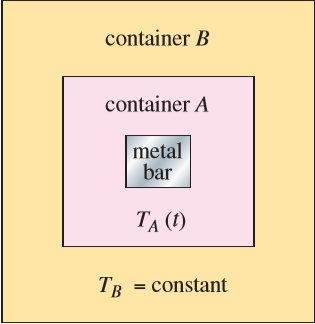
\includegraphics[width=0.7\linewidth]{assets/newton_cooling_law}
    \end{textblock*}
\end{frame}
%
%
%
\begin{frame}
    \frametitle{Formulation of SDE: $DTMC \to CTMC + ME \to SDE$}
%
        \begin{textblock*}{60mm}(5mm, 15mm)
            A stochastic analogy.
            \begin{enumerate}[i)]
                \item
                    Formulate a discrete  stochastic model for the 
                dynamical system under study, which describe
                changes in a small time interval $\Delta t$
                \item
                    Compute the expected value and covariance for the change in 
                    a small time $\Delta$
                \item
                    Letting $\Delta t \to 0$, the above information leads to 
                    the a CTMC
                \item
                    Thus, we infer the SDE from the similarities in the 
                    forward backward Kolmogorov equation between  the discrete 
                    and Continuous Markov Chain
            \end{enumerate}
        \end{textblock*}
\end{frame}
%
\begin{frame}% frame 00
    \frametitle{Example: Formulation of a stochastic SIS model}
    \begin{textblock*}{50mm}(5mm, 10mm)
    Consider the deterministic SI model:
        \begin{align*}
            \frac{dS}{dt} &= -\frac{\beta}{N} S I + (b +\gamma) I
                \\
            \frac{dI}{dt} &= \frac{\beta}{N} S I - (b +\gamma) I
                \\
            N &= S(t)+ I(t)
        \end{align*}
        Where $N$ is constant and  $S(t) = N - I(t)$.
    \end{textblock*}
    \begin{textblock*}{50 mm}(60mm, 10mm)
        \begin{empheq}[box=\shadowbox]{align*}
            \mathcal{R}_0 &= 
                \frac{\beta}{b + \gamma}
                \\
            \mathcal{R}_0 & \leq 1
            \\
            & \Rightarrow
                \lim_{t \to \infty} (S(t),N(t)) = (N, 0)
            \\
            \mathcal{R}_0 & > 1
            \\
            & \Rightarrow
                \lim_{t \to \infty} (S(t),N(t)) = (N, 0)
        \end{empheq}
    \end{textblock*}
\end{frame}
%
%
%
\begin{frame}{Example: Formulation of a stochastic SIS model}
    \begin{textblock*}{55mm}(5mm, 10mm)
        Consider the process $\{\mathcal{I}_t\}_{t=0} ^ \infty$ with 
        time discrete and space of states $\{0,1,\cdots, N \}$.
        \begin{enumerate}[(H-1)]
            \item
                $
                    \{\mathcal{I}_t\}_{t=0} ^ \infty
                $ define
                \begin{align*}
                    p_i(t) &:= \probX{\mathcal{I}(t) = i}
                    \\
                    i &= 0,1,2\dots,
                    \\
                    t &= 0, \Delta t, 2 \Delta t, \cdots,
                \end{align*}
            \item
                Markov property
                $$
                    \probCX{I_{t + \Delta t}}{  I_0, I_{\Delta t}, \cdots, I_t}
                    =\probCX{I_{t + \Delta t} }{I_t}
                $$
            \item
                The unique transitions with positive 
                probability
                \begin{align*}
                    & p_{ji}(t + \Delta t)
                    = 
                    \probCX{I_{t + \Delta t} = j}{I_t = i}
                    \\
                    &\text{are}
                    \\
                    & i \to i+1, \ i \to i-1,  \ i \to i
                \end{align*}
        \end{enumerate}
%
%
%
        \begin{textblock*}{50mm}(55mm, 10mm)
            \begin{equation*}
                p_{ji}(\Delta t):=
                    \begin{cases}
                        \frac{\beta i (N - i)}{N} \Delta t, 
                            & j = i + 1
                        \\
                        (b + \gamma) i \Delta t, 
                            & j = i - 1
                        \\
                        1 - 
                        \left[
                            \frac{\beta i (N - i)}{N} +
                            (b + \gamma) i
                        \right]
                        \Delta t, 
                            & j=i,
                        \\
                        0 & \text{otherwise}
                \end{cases}
            \end{equation*}
            where $\Delta t$ is sufficient small s.t.
            $$
                \max_{i \in \{ 1, \dots, N \}}
                \{
                    [b(i) + d(i)] \Delta t
                \}
                \leq 1
            $$
        \end{textblock*}
%
        \begin{textblock*}{50mm}(65mm, 60mm)
            \begin{center}
                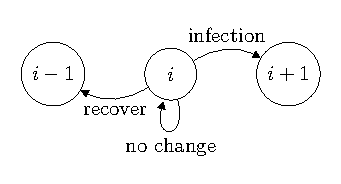
\includegraphics[width=\linewidth]{assets/chain.pdf}
            \end{center}
        \end{textblock*}
    \end{textblock*}
\end{frame}
%%%%%%%%%%%%%%%%%%%%%%%%%%%%%%%%%%%%%%%%%%%%%%%%%%%%%%%%%%%%%%%%%%%%%%%%%%%%%%%%
\begin{frame}{Example: Formulation of a stochastic SIS model}
    \begin{textblock*}{55mm}(5mm, 10mm)
        Letting
        \begin{align*}
            b(i) &:= \frac{\beta i (N - i)}{N} \Delta t
            \\
            d(i) &:= (b + \gamma) i \Delta t
        \end{align*}
        Thus $P(\Delta t) = $
    \end{textblock*}
    \begin{textblock*}{90mm}(45mm, 8mm)
        \begin{empheq}[box={\Garybox[FKE]}]{align*}
            p_i(t + \Delta t) &=
                p_{i-1}(t) b(i - 1) \Delta t 
                \\
                & + p_{i+1}(t) d(i + 1) \Delta t
                \\
                & + p_i(t) (1 -[b(i) + d(i)] \Delta t)
        \end{empheq}
    \end{textblock*}

    \begin{textblock*}{140mm}(-3mm, 35mm)
        %
        \begin{equation*}
            \begin{pmatrix}
            1   & d(1) \Delta t & 0 & \cdots    & 0 & 0
            \\
            0   & 1 - (b+d)(1) \Delta t & d(2)  \Delta t   & \cdots    & 0   & 
            0 
            \\
            0   & b(1) \Delta t  & 1 - (b+d)(2) \Delta t   & \cdots    & 0 & 0
            \\
            0 & 0 & b(2) \Delta t & \cdots    & 0 & 0
            \\
            \vdots & \vdots & \vdots & \ddots & \vdots & \vdots
            \\
            0 & 0 & 0 & \cdots & d (N - 1) \Delta t  & 0
            \\
            0 & 0 & 0 & \cdots & 1- (b+d) (N - 1) \Delta t  & d(N) \Delta t
            \\
            0 & 0 & 0 & \cdots & d (N - 1) \Delta t  &  1 - d(N) \Delta t 
            \end{pmatrix}
        \end{equation*}
        \begin{textblock*}{100mm}(10mm, 80mm)
            $$
                p(t + \Delta t) = P(\Delta t) p(t) = P^{n+1}(\Delta t) p(0), 
                \qquad t =n \Delta t
            $$
        \end{textblock*}
    \end{textblock*}
%
\end{frame}
%
%
\begin{frame}{Expected Value of the SIS-DTMC}
    \begin{textblock*}{80mm}(0mm,10mm)
        \begin{align*}
            \E(I_{t + \Delta t}) &=  
                \sum_{i = 0} ^ N
                    i p_i(t + \Delta t)
            \\
                &=
                    \sum_{i = 0} ^ N
                        i p_{i - 1} (t) b(i - 1) \Delta t
                   + \sum_{i = 0} ^ {N-1}
                        i p_{i + 1} (t) d(i + 1) \Delta t
            \\
                & + \sum_{i=0}^N i p_i(t) \Delta t
                - \sum_{i=0}^N i p_i(t) b(i) \Delta t
                - \sum_{i=0}^N i p_i(t) d(i) \Delta t
            \\
                \E(I_{t+ \Delta t}) 
                &= 
                    \E(I_t) 
                        + \sum_{i = 1} ^ N
                        p_{i-1} (t)
                        \frac{\beta (i-1)(N - [i -1])}{N} \Delta t
            \\
                    &-
                        \sum_{i = 0} ^ {N - 1}
                        p_{i + 1} (t) (b + \gamma) (i+1) \Delta t
            \\
                &=
                \E(I_t) + [\beta - (b + \gamma )] \Delta t \E(I_t)
                -\frac{\beta}{N} \Delta t 
                \underbrace{\E(I_t ^ 2)}_{\geq \E ^2(I_t)}
        \end{align*}
    \end{textblock*}
%
%
%
\end{frame}
%%%%%%%%%%%%%%%%%%%%%%%%%%%%%%%%%%%%%%%%%%%%%%%%%%%%%%%%%%%%%%%%%%%%%%%%%%%%%%%%
\begin{frame}{Expected Value of the SIS-DTMC}
    \begin{textblock*}{60mm}(10mm, 10mm)
       \begin{equation*}
            \frac{\E(I_{t + \Delta t}) - \E(I_t)}{\Delta t}
                \leq
                    [\beta  - (b + \gamma)] \E (I_t)
                    - \frac{\beta}{N} \E^2 (I_t)
        \end{equation*}
        %
        \begin{align*}
            \frac{d \E(I_{t})}{dt}
                & \leq
                    [\beta  - (b + \gamma)] \E (I_t)
                    - \frac{\beta}{N} \E ^ 2 (I_t)
            \\
                & = \frac{\beta}{N} [N - \E(I_t)] \E (I_t)
                    - (b + \gamma) \E (I_t)
        \end{align*}
        \begin{empheq}[box=\shadowbox]{equation*}
            \frac{d \E(I_{t})}{dt}
            \leq
            \frac{\beta}{N} \E(S_t) \E (I_t)
                - (b + \gamma) \E (I_t)
        \end{empheq}
    \end{textblock*}
\end{frame}

%%%%%%%%%%%%%%%%%%%%%%%%%%%%%%%%%%%%%%%%%%%%%%%%%%%%%%%%%%%%%%%%%%%%%%%%%%%%%%%%
\begin{frame}{Example: Formulation of a stochastic SIS model}
    \begin{textblock*}{55mm}(5mm, 10mm)
        \begin{empheq}[box=\shadowbox]{align*}
            N &= 100, \ \Delta t = 0.01, \ \beta = 1, 
            \\
            b &= 0.25 \ \gamma = 0.25 
        \end{empheq}
    \end{textblock*}
%
    \begin{textblock*}{100mm}(5mm, 20mm)
        \begin{center}
            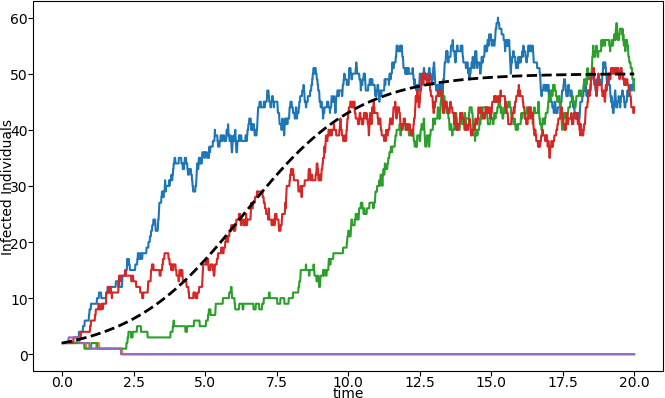
\includegraphics[width=\linewidth]{assets/random_walk_SIS}
        \end{center}
    \end{textblock*}
%
    \begin{textblock*}{20mm}(105mm, 20mm)
        \begin{empheq}[box=\fbox]{align*}
            \mathcal{R}_0 &= 2,  
             \\
            \bar{I} &= 50
        \end{empheq}
    \end{textblock*}
\end{frame}
%
\begin{frame}{}
    \begin{empheq}[box=\fbox]{align*}
        FKE:  &\frac{dp}{dt} = Q p
        \\
        p(t) & = (p_0(t), \dots, p_N(t)) ^ {\top}
    \end{empheq}
    \begin{equation*}
        Q = 
        \begin{pmatrix}
            0   & d(1)  & 0 & \dots     & 0
            \\
            0   & -[b(1) + d(1)]    & d(2)  & \dots     & 0
            \\
            0   & b(1)  & -[b(2) + d(2)]    & \dots     & 0     
            \\
            0   & 0     & b(2)  & \dots     & 0
            \\
            \vdots  & \vdots    & \vdots    & \ddots    & \vdots
            \\
            0   & 0     & 0     & \dots     & d(N)
            \\
            0   & 0     & 0     & \dots     & -d(N)    
        \end{pmatrix}
    \end{equation*}
    Results that
    $$
        \lim_{t \to \infty}
            p(t) = (1, 0, \dots, 0)^{\top}
    $$
    and
    $$
        Q = \lim_{\Delta t \to 0}
            \frac{P(\Delta t) - I}{\Delta t}
    $$
\end{frame}
%
%
        
    \section{Continuous Time Markov Chains (CTMC}
            \begin{frame}{Formulating a SIS-CTMC }
        Let 
        \begin{align*}
            & \{ I_t\}_{t \geq 0},
            \\
            & p_i(t) = \probX{I_t = i}.
        \end{align*}
        Thus, the Markov porperty becomes in
        \begin{align*}
            \probCX{ I_{t_{n + 1}}}{I_{t_0}, \cdots, I_{t_n} }
                &=
                \probCX{ I_{t_{n + 1}}}{I_{t_n}}
                \\
                \text{for all } &
                t_0 < t_1 < \cdots < t_n 
        \end{align*}
        \begin{align*}
            &p_{ji}(\Delta t):=
                \begin{cases}
                    \frac{\beta i (N - i)}{N} \Delta t 
                        + o(\Delta t),     
                        & j = i + 1
                    \\
                    (b + \gamma) i \Delta t 
                        + o(\Delta t),
                        &   j = i - 1
                    \\
                    1 - \left [
                            \frac{\beta i (N - i)}{N} +
                            (b + \gamma) i %                
                        \right] \Delta t
                        + o(\Delta t) , 
                        & j=i
                    \\
                    o(\Delta t) & \text{otherwise}
                \end{cases}
            \\
            & \lim_{t\to \infty}
                \frac{o(\Delta t)}{\Delta t}
                = 0
        \end{align*}
    \end{frame}
 %%%%%%%%%%%%%%%%%%%%%%%%%%%%%%%%%%%%%%%%%%%%%%%%%%%%%%%%%%%
    \begin{frame}{}
        Using the notation for birth and death
        processes, we have

        \begin{equation*}
            p_{ij}(\Delta t):=
                \begin{cases}
                    b(i) \Delta t + o(\Delta t),     
                        & j = i + 1
                    \\
                    d(i) \Delta t + o(\Delta t), 
                        &   j = i - 1
                    \\
                    1 - \left [
                            b(i) + d(i) %                
                        \right] \Delta t
                        + o(\Delta t), 
                        & j=i
                    \\
                    0 & \text{otherwise}
                \end{cases}
        \end{equation*}
        Assuming $\probX{I_0 = i_0} = 1$, then
        \begin{align*}
            p_i(t + \Delta t)
                =&
                    p_{i - 1} (t) b(i -1) \Delta t
                    \\
                    & + 
                        p_{i + 1} (t) d(i + 1) \Delta t
                    \\
                    & +
                        p_{i} (t)[1 - (b(i) + d(i))] \Delta t
                    + o(\Delta t)
            \\
            i &= 1, 2, \dots, N
        \end{align*}
    \end{frame}
    \section{Brownian Motion}
    
    \section{Poisson Process}
    \section{Choosing a noise processes}
        \begin{frame}{Stochastic Processes in Biology}
        
        \end{frame}
    \section{Open Problems}
\end{document}
